\documentclass[11pt,a4paper]{article}

\usepackage[utf8]{inputenc}
\usepackage[T1]{fontenc}
\usepackage{amsmath,amssymb}
\usepackage{graphicx}
\usepackage{booktabs}
\usepackage[margin=2.5cm]{geometry}
\usepackage{hyperref}

\graphicspath{{../results/}}

\title{Economic Dispatch and DC Optimal Power Flow\\on the IEEE 30-Bus System}
\author{%
  Rishabh Roy Choudhury \and
  Varshith Tadiparthi \and
  B.~Rithwik\\[4pt]
  \textit{Team Albert and Einstein}
}
\date{November 2026}

\begin{document}
\maketitle

\begin{abstract}
We formulate the Economic Dispatch (ED) and DC Optimal Power Flow (DC-OPF)
problems as convex quadratic programs on the IEEE 30-bus test system and solve
them with two custom solvers: a lambda-iteration (bisection) method for ED and
a primal active-set method (Nocedal and Wright, Algorithm~16.3) for general QPs.
Both are validated against a CVXPY + Clarabel reference.  We show that the
Lagrange multipliers of the power-balance constraints are Locational Marginal
Prices (LMPs), equal at every bus until line congestion causes them to separate.
\end{abstract}

% TODO Rishabh: formulation section
% \section{Problem Statement and Mathematical Formulation}
\label{sec:formulation}

\subsection{Motivation and Overview}
In modern wholesale electricity markets, the system transmission operator must schedule generator outputs to satisfy aggregate consumer demand at the lowest possible operating cost, subject to technical constraints on generator capacities and network power flows. When transmission lines have ample thermal capacity, economic efficiency dictates that all generators operate at equal incremental cost---a problem known as Economic Dispatch (ED) \cite{wood2014}. However, in physical transmission grids, line flow ratings frequently constrain the transfer of low-cost generation to load centers. This requires the operator to solve the DC Optimal Power Flow (DC-OPF) problem, redispatching more expensive local units to prevent line overloads \cite{wood2014, zimmerman2011}.

Crucially, the dual Lagrange multipliers associated with the bus real power balance equations correspond to Locational Marginal Prices (LMPs) \cite{boyd2004}. When lines are uncongested, LMPs are uniform across the entire grid. Under transmission congestion, LMPs separate across buses, reflecting the local marginal cost of supplying an incremental megawatt of power while respecting transmission boundaries.

\subsection{System Data and Notation}
We evaluate both formulations on the standard IEEE 30-bus test system from MATPOWER \cite{zimmerman2011}, consisting of 30 buses, 6 generating units, and 41 transmission branches, with an aggregate active load of $D = 189.20\text{ MW}$ and base power $S_{\text{base}} = 100\text{ MVA}$. Table~\ref{tab:notation} summarizes the mathematical notation, and Table~\ref{tab:generator_data} lists the technical parameters and quadratic cost coefficients for all six generators parsed from \texttt{data/case30.m}.

\begin{table}[htbp]
\centering
\caption{Mathematical notation for ED and DC-OPF.}
\label{tab:notation}
\begin{tabular}{ll}
\toprule
Symbol & Description \\
\midrule
$n_{\text{bus}}, n_{\text{gen}}, n_{\text{branch}}$ & Number of buses (30), generators (6), and branches (41) \\
$S_{\text{base}}$ & System base power (100.0 MVA) \\
$P_i$ & Active power output of generator $i$ (MW) \\
$\theta_k$ & Voltage phase angle at bus $k$ (radians) \\
$d_k$ & Real power demand at bus $k$ (MW) \\
$b_i, c_i$ & Linear (\$/MWh) and quadratic (\$/MW$^2$h) generator cost coefficients \\
$P_{\min, i}, P_{\max, i}$ & Minimum and maximum generation limits (MW) \\
$x_l$ & Series reactance of branch $l$ (per unit) \\
$F_{\max, l}$ & Long-term rating (RATE\_A) of branch $l$ (MW/MVA) \\
$C_g \in \mathbb{R}^{30 \times 6}$ & Generator-to-bus incidence matrix \\
$C \in \mathbb{R}^{41 \times 30}$ & Branch-to-bus incidence matrix ($+1$ at from-bus, $-1$ at to-bus) \\
$B_{\text{bus}} \in \mathbb{R}^{30 \times 30}$ & Bus susceptance matrix, $B_{\text{bus}} = C^T \operatorname{diag}(1/x) C$ \\
$\lambda \in \mathbb{R}^{31}$ & Dual multipliers for equality constraints (LMPs and reference row) \\
$\mu \in \mathbb{R}^{94}$ & Dual multipliers for inequality constraints (lines and generators) \\
\bottomrule
\end{tabular}
\end{table}

\begin{table}[htbp]
\centering
\caption{Generator cost coefficients, operational limits, and bus locations (IEEE 30-bus system).}
\label{tab:generator_data}
\begin{tabular}{crrrrr}
\toprule
Generator $i$ & Bus & $P_{\min, i}$ (MW) & $P_{\max, i}$ (MW) & $b_i$ (\$/MWh) & $c_i$ (\$/MW$^2$h) \\
\midrule
1 & 1  & 0.0 & 80.0 & 2.000 & 0.02000 \\
2 & 2  & 0.0 & 80.0 & 1.750 & 0.01750 \\
3 & 22 & 0.0 & 50.0 & 1.000 & 0.06250 \\
4 & 27 & 0.0 & 55.0 & 3.250 & 0.00834 \\
5 & 23 & 0.0 & 30.0 & 3.000 & 0.02500 \\
6 & 13 & 0.0 & 40.0 & 3.000 & 0.02500 \\
\bottomrule
\end{tabular}
\end{table}

\subsection{Economic Dispatch Formulation}
The Economic Dispatch problem ignores network transmission constraints and minimizes the total quadratic operating cost subject only to system-wide power balance and individual generator capacity limits:
\begin{align}
    \min_{P \in \mathbb{R}^6} \quad & \sum_{i=1}^{n_{\text{gen}}} \left( b_i P_i + c_i P_i^2 \right) \label{eq:ed_obj} \\
    \text{subject to} \quad & \sum_{i=1}^{n_{\text{gen}}} P_i = \sum_{k=1}^{n_{\text{bus}}} d_k \cdot \text{load\_scale} \label{eq:ed_balance} \\
    & P_i \le P_{\max, i}, \quad \forall i \in \{1, \dots, n_{\text{gen}}\} \label{eq:ed_pmax} \\
    & -P_i \le -P_{\min, i}, \quad \forall i \in \{1, \dots, n_{\text{gen}}\} \label{eq:ed_pmin}
\end{align}
In the canonical QP format of \texttt{src/opf/models.py}, the ED problem has $n = 6$ primal variables, $m_{\text{eq}} = 1$ equality constraint ($A_{\text{eq}} = \mathbf{1}_{1 \times 6}$), and $m_{\text{in}} = 12$ inequality constraints ($A_{\text{in}} = \begin{bmatrix} I_6 \\ -I_6 \end{bmatrix}$).

\subsection{DC Optimal Power Flow Formulation}
The DC-OPF model incorporates transmission network physics under standard DC power flow assumptions \cite{wood2014}:
\begin{enumerate}
    \item Transmission lines are lossless (branch resistance $r \ll x$ is neglected).
    \item Voltage magnitudes are constant at $1.0\text{ p.u.}$ across all buses.
    \item Voltage phase angle differences across lines are small ($\sin(\theta_i - \theta_j) \approx \theta_i - \theta_j$).
    \item Reactive power flows and voltage dependencies are uncoupled from real power flows.
\end{enumerate}

The primal optimization variable is $x = [P_1, \dots, P_6, \theta_1, \dots, \theta_{30}]^T \in \mathbb{R}^{36}$. The DC-OPF quadratic program is:
\begin{align}
    \min_{x \in \mathbb{R}^{36}} \quad & \frac{1}{2} x^T H x + g^T x = \sum_{i=1}^{n_{\text{gen}}} \left( b_i P_i + c_i P_i^2 \right) \label{eq:dcopf_obj} \\
    \text{subject to} \quad & C_g P - S_{\text{base}} B_{\text{bus}} \theta = d \cdot \text{load\_scale} \quad (30\text{ nodal balance rows}) \label{eq:dcopf_balance} \\
    & \theta_{\text{ref}} = \theta_1 = 0 \quad (1\text{ reference angle row}) \label{eq:dcopf_ref} \\
    & +S_{\text{base}} \operatorname{diag}(1/x) C \theta \le F_{\max} \cdot \text{rate\_scale} \quad (41\text{ forward line limits}) \label{eq:dcopf_line_fwd} \\
    & -S_{\text{base}} \operatorname{diag}(1/x) C \theta \le F_{\max} \cdot \text{rate\_scale} \quad (41\text{ reverse line limits}) \label{eq:dcopf_line_rev} \\
    & P_i \le P_{\max, i}, \quad \forall i \in \{1, \dots, 6\} \quad (6\text{ gen upper limits}) \label{eq:dcopf_gen_up} \\
    & -P_i \le -P_{\min, i}, \quad \forall i \in \{1, \dots, 6\} \quad (6\text{ gen lower limits}) \label{eq:dcopf_gen_lo}
\end{align}
As implemented in \texttt{build\_dcopf()}, this yields $n = 36$ decision variables, $m_{\text{eq}} = 31$ equality constraints, and $m_{\text{in}} = 94$ inequality constraints ($41 + 41 + 6 + 6 = 94$).

\subsection{Convexity and KKT Optimality Conditions}
The objective Hessian is $H = \begin{bmatrix} \operatorname{diag}(2c) & 0 \\ 0 & 0_{30 \times 30} \end{bmatrix}$. Because $c_i > 0$ for all generators, $\operatorname{diag}(2c)$ is strictly positive definite on the generation subspace $P$, and zero on $\theta$. Thus $H$ is symmetric positive semidefinite ($H \succeq 0$), ensuring that the quadratic cost function is convex \cite{boyd2004}. Furthermore, all 31 equality constraints and 94 inequality constraints are linear, defining a polyhedral convex feasible set. By convex optimization theory \cite{boyd2004, nocedal2006}, any local solution is a global optimum, and the Karush-Kuhn-Tucker (KKT) conditions are both necessary and sufficient for global optimality.

\subsection{Susceptance Matrix Singularity and Reference Bus}
Each row of the branch-bus incidence matrix $C$ contains exactly one $+1$ and one $-1$, which implies $C \mathbf{1} = 0$, where $\mathbf{1}$ is the all-ones vector. Consequently:
\begin{equation}
    B_{\text{bus}} \mathbf{1} = C^T \operatorname{diag}(1/x) C \mathbf{1} = 0
\end{equation}
For any connected network, the nullspace of $B_{\text{bus}}$ is exactly $\operatorname{span}(\mathbf{1})$, meaning $B_{\text{bus}}$ has rank $n_{\text{bus}} - 1 = 29$. Without an angular reference, the nodal balance equations (\ref{eq:dcopf_balance}) are invariant under an arbitrary global shift $\theta \leftarrow \theta + \phi \mathbf{1}$. Fixing the reference angle $\theta_{\text{ref}} = \theta_1 = 0$ removes this degree of freedom and makes the 31 rows of $A_{\text{eq}}$ linearly independent (full row rank).

\subsection{KKT Multipliers and Locational Marginal Prices}
Under our project's Lagrangian definition:
\begin{equation}
    \mathcal{L}(x, \lambda, \mu) = \frac{1}{2} x^T H x + g^T x - \lambda^T (A_{\text{eq}} x - b_{\text{eq}}) + \mu^T (A_{\text{in}} x - b_{\text{in}})
\end{equation}
the KKT stationarity condition is:
\begin{equation}
    \nabla_x \mathcal{L} = H x + g - A_{\text{eq}}^T \lambda + A_{\text{in}}^T \mu = 0
\end{equation}
together with primal feasibility ($A_{\text{eq}} x = b_{\text{eq}}$, $A_{\text{in}} x \le b_{\text{in}}$), dual feasibility ($\mu \ge 0$), and complementary slackness ($\mu_j (a_{\text{in}, j}^T x - b_{\text{in}, j}) = 0$).

By the sensitivity theorem of convex programming \cite{boyd2004}, the vector of equality multipliers $\lambda$ satisfies:
\begin{equation}
    \lambda_k = \frac{\partial q^*}{\partial b_{\text{eq}, k}}
\end{equation}
Because the first 30 equality rows correspond to bus real power balance $b_{\text{eq}, k} = d_k$, multiplier $\lambda_k$ ($k=1,\dots,30$) is the exact marginal cost of supplying an incremental megawatt of load at bus $k$---the Locational Marginal Price (the LMPs are positive in all our test cases). Row 31 corresponds to $\theta_1 = 0$, whose multiplier $\lambda_{31} \approx 0$ enforces the reference angle and carries no price interpretation.

\subsection{Worked Base-Case Check: Equal Marginal Costs}
When the transmission network is uncongested (base case with $\text{rate\_scale} = 1.0$), no transmission constraints or generator bounds are active ($\mu = 0$). Differentiating the Lagrangian with respect to generator output $P_i$ located at bus $k$ yields:
\begin{equation}
    \frac{\partial \mathcal{L}}{\partial P_i} = b_i + 2 c_i P_i - \lambda_k = 0 \implies \text{MC}_i = b_i + 2 c_i P_i = \lambda_k
\end{equation}
Evaluating this marginal cost check at the optimal base-case dispatch from our solver:
\begin{itemize}
    \item Generator 1 ($P_1 = 44.7299\text{ MW}$): $\text{MC}_1 = 2.000 + 2(0.02000)(44.7299) = 3.7892\text{ \$/MWh}$
    \item Generator 2 ($P_2 = 58.2628\text{ MW}$): $\text{MC}_2 = 1.750 + 2(0.01750)(58.2628) = 3.7892\text{ \$/MWh}$
    \item Generator 3 ($P_3 = 22.3136\text{ MW}$): $\text{MC}_3 = 1.000 + 2(0.06250)(22.3136) = 3.7892\text{ \$/MWh}$
    \item Generator 4 ($P_4 = 32.3259\text{ MW}$): $\text{MC}_4 = 3.250 + 2(0.00834)(32.3259) = 3.7892\text{ \$/MWh}$
    \item Generator 5 ($P_5 = 15.7839\text{ MW}$): $\text{MC}_5 = 3.000 + 2(0.02500)(15.7839) = 3.7892\text{ \$/MWh}$
    \item Generator 6 ($P_6 = 15.7839\text{ MW}$): $\text{MC}_6 = 3.000 + 2(0.02500)(15.7839) = 3.7892\text{ \$/MWh}$
\end{itemize}
All six generators operate at an identical marginal cost of $3.7892\text{ \$/MWh}$, precisely matching the system LMP across all 30 buses.


% methods.tex: Optimization Methods and Algorithms
% Author: Varshith Tadiparthi (Albert and Einstein)
% Workstream: Solvers (Economic Dispatch & Primal Active-Set QP)

\section{Optimization Methods and Numerical Solvers}
\label{sec:methods}

To solve the Economic Dispatch (ED) and DC Optimal Power Flow (DC-OPF) convex quadratic programs, we implemented two independent, exact numerical solvers. The iterations of both solvers use only NumPy without relying on external QP optimization packages. The only use of \texttt{scipy.optimize.linprog} is inside \texttt{feasible\_start()} purely to find a feasible starting point when the economic-dispatch candidate violates a line limit:
\begin{enumerate}
    \item \textbf{Lambda-Iteration (Bisection) Solver} for Economic Dispatch (\path{src/opf/lambda_iteration.py}).
    \item \textbf{Primal Active-Set Quadratic Programming Solver} (Nocedal and Wright, Algorithm 16.3) for both ED and network-constrained DC-OPF (\path{src/opf/active_set.py}).
\end{enumerate}

\subsection{Economic Dispatch via Lambda-Iteration}

\subsubsection{KKT Optimality and Decoupled Dispatch}
The classical Economic Dispatch problem minimizes the total generator operating cost subject to power balance and capacity limits:
\begin{align}
    \min_{\{P_i\}} \quad & \sum_{i=1}^n \left( c_i P_i^2 + b_i P_i \right) \label{eq:ed_obj} \\
    \text{subject to} \quad & \sum_{i=1}^n P_i = D \quad (\lambda) \label{eq:ed_bal} \\
    & P_i^{\min} \le P_i \le P_i^{\max}, \quad \forall i = 1, \dots, n \label{eq:ed_bounds}
\end{align}
where $c_i > 0$ ensures strict convexity.

Under the project sign convention, the Lagrangian function is defined as:
\begin{equation}
\begin{split}
    \mathcal{L}(P, \lambda, \mu^+, \mu^-) = \; & \sum_{i=1}^n (c_i P_i^2 + b_i P_i) - \lambda \left(\sum_{i=1}^n P_i - D\right) \\
    & + \sum_{i=1}^n \mu_i^+ (P_i - P_i^{\max}) + \sum_{i=1}^n \mu_i^- (P_i^{\min} - P_i)
\end{split}
\end{equation}
with dual multipliers $\mu_i^+ \ge 0$ and $\mu_i^- \ge 0$.

The Karush-Kuhn-Tucker (KKT) first-order optimality conditions are:
\begin{enumerate}
    \item \textbf{Stationarity:}
    \begin{equation}
        \frac{\partial \mathcal{L}}{\partial P_i} = 2 c_i P_i + b_i - \lambda + \mu_i^+ - \mu_i^- = 0 \implies 2 c_i P_i + b_i = \lambda - \mu_i^+ + \mu_i^-
    \end{equation}
    \item \textbf{Primal Feasibility:} Constraints (\ref{eq:ed_bal}) and (\ref{eq:ed_bounds}) hold.
    \item \textbf{Dual Feasibility:} $\mu_i^+ \ge 0, \; \mu_i^- \ge 0$.
    \item \textbf{Complementary Slackness:}
    \begin{equation}
        \mu_i^+ (P_i - P_i^{\max}) = 0, \quad \mu_i^- (P_i^{\min} - P_i) = 0
    \end{equation}
\end{enumerate}

From complementary slackness, for any trial system marginal price $\lambda$:
\begin{itemize}
    \item If $P_i^{\min} < P_i < P_i^{\max}$, then $\mu_i^+ = \mu_i^- = 0$, yielding the \textit{equal incremental cost rule}:
    \begin{equation}
        \text{IC}_i(P_i) = 2 c_i P_i + b_i = \lambda \implies P_i(\lambda) = \frac{\lambda - b_i}{2 c_i}
    \end{equation}
    \item If $P_i = P_i^{\max}$, then $\mu_i^- = 0$ and $\mu_i^+ = \lambda - (2 c_i P_i^{\max} + b_i) \ge 0 \implies \lambda \ge 2 c_i P_i^{\max} + b_i$.
    \item If $P_i = P_i^{\min}$, then $\mu_i^+ = 0$ and $\mu_i^- = (2 c_i P_i^{\min} + b_i) - \lambda \ge 0 \implies \lambda \le 2 c_i P_i^{\min} + b_i$.
\end{itemize}

Combining all three regimes yields the exact closed-form decoupled generator response:
\begin{equation}
    P_i(\lambda) = \operatorname{clip}\left( \frac{\lambda - b_i}{2 c_i}, \; P_i^{\min}, \; P_i^{\max} \right)
\end{equation}

\subsubsection{Monotonicity, Bracketing, and Bisection Algorithm}
Since $c_i > 0$, each individual generator characteristic $P_i(\lambda)$ is continuous and monotonically non-decreasing in $\lambda$. Consequently, the total power output function:
\begin{equation}
    P_{\text{total}}(\lambda) = \sum_{i=1}^n P_i(\lambda)
\end{equation}
is also continuous and monotonically non-decreasing.

The root-finding problem $h(\lambda) = P_{\text{total}}(\lambda) - D = 0$ is bounded by natural physical brackets:
\begin{equation}
    \lambda_{\min} = \min_{1 \le i \le n} \left( b_i + 2 c_i P_i^{\min} \right), \quad \lambda_{\max} = \max_{1 \le i \le n} \left( b_i + 2 c_i P_i^{\max} \right)
\end{equation}
where $P_{\text{total}}(\lambda_{\min}) = \sum P_i^{\min}$ and $P_{\text{total}}(\lambda_{\max}) = \sum P_i^{\max}$.

\paragraph{Infeasibility Criterion:} If $D < \sum P_i^{\min} - \epsilon$ or $D > \sum P_i^{\max} + \epsilon$, no feasible generation schedule exists; the solver immediately returns status \texttt{"infeasible"}.

\paragraph{Convergence:} At each iteration $k$, the midpoint $\lambda_k = \frac{1}{2}(\lambda_{\text{low}} + \lambda_{\text{high}})$ is evaluated. The interval width contracts geometrically:
\begin{equation}
    |\lambda_{\text{high}}^{(k)} - \lambda_{\text{low}}^{(k)}| = \frac{1}{2^k} |\lambda_{\max} - \lambda_{\min}|
\end{equation}
Iteration terminates when the power balance residual satisfies $|P_{\text{total}}(\lambda_k) - D| \le \text{tol}$.

\subsection{Primal Active-Set Quadratic Programming Solver}

For problems with general linear inequality constraints (such as line flow ratings in DC-OPF), decoupling is not possible. We implemented the Primal Active-Set Method following Nocedal and Wright (Algorithm 16.3).

\subsubsection{Standard QP Formulation}
The general convex QP is expressed as:
\begin{align}
    \min_{x \in \mathbb{R}^n} \quad & q(x) = \frac{1}{2} x^T H x + g^T x \\
    \text{subject to} \quad & A_{eq} x = b_{eq} \\
    & A_{in} x \le b_{in}
\end{align}

\subsubsection{Working Set and KKT Equality Subproblem}
At iteration $k$ with feasible iterate $x_k$, let $\mathcal{W}_k \subseteq \{1, \dots, m_{in}\}$ denote the \textit{working set} of active inequality constraints treated as equalities ($A_{in}[\mathcal{W}_k] x_k = b_{in}[\mathcal{W}_k]$).

To compute a step $p_k = x_{k+1} - x_k$ that minimizes $q(x_k + p)$ on the working manifold, we solve the equality-constrained subproblem:
\begin{align}
    \min_{p} \quad & \frac{1}{2} p^T H p + g_k^T p \\
    \text{subject to} \quad & A_{eq} p = 0 \\
    & A_{\mathcal{W}} p = 0
\end{align}
where $g_k = \nabla q(x_k) = H x_k + g$, and $A_{\mathcal{W}} = A_{in}[\mathcal{W}_k, :]$.

Under our project's Lagrangian convention:
\begin{equation}
    \mathcal{L}(x, \lambda, \mu) = \frac{1}{2} x^T H x + g^T x - \lambda^T (A_{eq} x - b_{eq}) + \mu^T (A_{in} x - b_{in})
\end{equation}
stationarity at the subproblem solution requires:
\begin{equation}
    H p + g_k - A_{eq}^T \lambda + A_{\mathcal{W}}^T \mu_{\mathcal{W}} = 0 \implies H p - A_{eq}^T \lambda + A_{\mathcal{W}}^T \mu_{\mathcal{W}} = -g_k
\end{equation}
Assembling the full Karush-Kuhn-Tucker system into block matrix form:
\begin{equation}
    \begin{bmatrix}
        H & -A_{eq}^T & A_{\mathcal{W}}^T \\
        A_{eq} & 0 & 0 \\
        A_{\mathcal{W}} & 0 & 0
    \end{bmatrix}
    \begin{bmatrix}
        p \\
        \lambda \\
        \mu_{\mathcal{W}}
    \end{bmatrix}
    =
    \begin{bmatrix}
        -g_k \\
        0 \\
        0
    \end{bmatrix}
    \label{eq:kkt_system}
\end{equation}
The $-A_{eq}^T$ block ensures that the equality multiplier $\lambda$ matches the economic definition of Locational Marginal Prices ($\lambda > 0$), while $+A_{\mathcal{W}}^T$ directly computes non-negative dual variables $\mu_{\mathcal{W}} \ge 0$ for active inequality constraints.

\subsubsection{Algorithmic Flow (Algorithm 16.3)}
\begin{enumerate}
    \item \textbf{Initialization and Rank Verification:}
    Start from a primal feasible point $x_0$ (obtained via \texttt{feasible\_start()}, which uses \texttt{scipy.optimize.linprog} strictly if the unconstrained ED candidate violates line limits). The active-set iterations themselves use only NumPy. Active inequality constraints ($|a_i^T x_0 - b_i| \le \text{tol}$) are added to $\mathcal{W}_0$ one by one \textit{if and only if} they increase the row rank of $\begin{bmatrix} A_{eq} \\ A_{\mathcal{W}} \end{bmatrix}$. This prevents Linear Independence Constraint Qualification (LICQ) breakdown and singularity in system (\ref{eq:kkt_system}).

    \item \textbf{Step Evaluation ($p_k \approx 0$):}
    If $\|p_k\|_\infty \le \text{tol}$, $x_k$ is the exact minimizer on the current working subspace.
    \begin{itemize}
        \item If $\mu_i \ge -\text{tol}$ for all $i \in \mathcal{W}_k$, all KKT conditions are satisfied. \textbf{Declare optimality.}
        \item Otherwise, identify the constraint with the most negative multiplier:
        \begin{equation}
            j = \arg\min_{i \in \mathcal{W}_k} \mu_i
        \end{equation}
        Remove constraint $j$ from $\mathcal{W}_k$ and re-solve on the relaxed subspace without moving $x_k$.
    \end{itemize}

    \item \textbf{Ratio Test and Line Search ($p_k \neq 0$):}
    If $p_k \neq 0$, compute the maximum step length $\alpha_k \in [0, 1]$ that preserves primal feasibility across all inactive constraints ($i \notin \mathcal{W}_k$):
    \begin{equation}
        \alpha_k = \min \left( 1, \quad \min_{i \notin \mathcal{W}_k, \; a_i^T p_k > 0} \frac{b_i - a_i^T x_k}{a_i^T p_k} \right)
    \end{equation}
    Update $x_{k+1} = x_k + \alpha_k p_k$. If $\alpha_k < 1$, the step hit a boundary; add the blocking constraint (breaking ties by lowest index) to $\mathcal{W}_{k+1}$. A zero-length step ($\alpha_k = 0$) can occur when the iterate is at a vertex; the blocking constraint is still added to the working set.
\end{enumerate}

\subsubsection{Convergence and Numerical Properties}
Because the objective $q(x)$ is strictly decreasing at every nonzero step ($\alpha_k > 0$), and because there are only finitely many subsets $\mathcal{W} \subseteq \{1, \dots, m_{in}\}$, the algorithm terminates in a finite number of iterations in the absence of cycling. From the default \texttt{feasible\_start()} point the uncongested base case converges in one iteration, because that point is already the optimum; from a non-optimal \texttt{linprog} start it takes 13 iterations for the base case and 14 iterations for the congested case (rating $\times 0.75$).

\subsection{Economic Interpretation of Multipliers and Sensitivity Analysis}
\label{sec:lmp_sensitivity}

By the sensitivity theorem of nonlinear programming (Envelope Theorem), the optimal objective value function $q^*(b_{eq})$ satisfies:
\begin{equation}
    \nabla_{b_{eq}} q^*(b_{eq}) = \lambda
\end{equation}
For bus $k$, the equality constraint is the real power balance row:
\begin{equation}
    \sum_{i \text{ at } k} P_i - \sum_{l} f_{kl} = d_k \implies \frac{\partial q^*}{\partial d_k} = \lambda_k
\end{equation}
Thus, the dual multiplier $\lambda_k$ represents the exact marginal cost of supplying an incremental megawatt of power at bus $k$---the Locational Marginal Price (LMP).

\paragraph{Finite-Difference vs. Point Derivative:}
When evaluating a finite perturbation $\Delta d_k = 1.0\text{ MW}$, the change in optimal system cost $\Delta q^* = q^*(d + \Delta d) - q^*(d)$ differs from the point derivative $\lambda_k$ due to two effects:
\begin{enumerate}
    \item \textbf{Quadratic Cost Curvature:} Even when the optimal active set does not change, the cost function is strictly quadratic. Taylor expanding $q^*(d)$ around $d$:
    \begin{equation}
        q^*(d + \Delta d) = q^*(d) + \lambda_k \Delta d_k + \frac{1}{2} \left( \sum_{i=1}^n \frac{1}{2 c_i} \right)^{-1} (\Delta d_k)^2 + \mathcal{O}((\Delta d_k)^3)
    \end{equation}
    For the IEEE 30-bus base case with $\Delta d_k = 1.0\text{ MW}$, the second-order term evaluates to $\frac{1}{2} (0.006191)(1.0)^2 = +0.003096\text{ \$}$, perfectly accounting for the observed difference between the finite difference ($\Delta q^* = 3.792292\text{ \$}$) and the local derivative ($\lambda_k = 3.789196\text{ \$/MWh}$).
    \item \textbf{Active-Set Transitions:} When a generator or line limit becomes binding, the marginal price stays continuous but the slope of the price-demand curve changes (a kink), because the active set changes.
\end{enumerate}


\section{Results and Discussion}
\label{sec:results}

We evaluate the numerical accuracy, algorithmic efficiency, and physical implications of our optimization framework across a series of validation benchmarks and network stress sweeps on the IEEE 30-bus system.

\subsection{Solver Validation}

Table~\ref{tab:validation} compares our custom solvers (the primal active-set QP solver and the lambda-iteration bisection solver) against the CVXPY reference solver with the Clarabel backend across three standard benchmarks: uncongested DC-OPF (base case), congested DC-OPF (line ratings scaled to $0.75\times$), and Economic Dispatch (ED base).

\begin{table}[htbp]
\centering
\caption{Solver comparison: cost, primal/dual error vs.\ reference, KKT stationarity residual, and iteration counts (from default start and non-optimal start).}
\label{tab:validation}
\begin{tabular}{llrrrrrr}
\toprule
Solver & Scenario & Cost (\$/h) & $\max|\Delta x|$ & $\max|\Delta\lambda|$ & KKT res. & Iters & Iters (non-opt) \\
\midrule
reference & base & 565.21 & 0.00e+00 & 0.00e+00 & 8.31e-09 & 7 & --- \\
reference & rate\_0.75 & 565.97 & 0.00e+00 & 0.00e+00 & 2.06e-07 & 9 & --- \\
reference & ed\_base & 565.21 & 0.00e+00 & 0.00e+00 & 7.45e-07 & 6 & --- \\
active\_set & base & 565.21 & 4.27e-08 & 8.59e-10 & 2.40e-11 & 1 & 13 \\
active\_set & rate\_0.75 & 565.97 & 9.80e-06 & 8.86e-06 & 9.55e-12 & 9 & 14 \\
active\_set & ed\_base & 565.21 & 8.77e-07 & 4.00e-10 & 2.40e-11 & 1 & 11 \\
lambda\_iter & ed\_base & 565.21 & 8.77e-07 & 4.31e-10 & 5.07e-09 & 33 & --- \\
\bottomrule
\end{tabular}
\end{table}

Across all scenarios, our active-set solver agrees with the reference solution to high numerical precision. In the uncongested base case and ED problem, the active-set solver achieves primal errors $\max |\Delta x| \le 4.27 \times 10^{-8}$ and dual errors $\max |\Delta \lambda| \le 8.59 \times 10^{-10}$, with KKT stationarity residuals on the order of $10^{-11}$. In the congested scenario (ratings $\times 0.75$), the active-set solver matches the reference solution with primal deviation $\max |\Delta x| = 9.80 \times 10^{-6}$, dual deviation $\max |\Delta \lambda| = 8.86 \times 10^{-6}$, and KKT residual $9.55 \times 10^{-12}$. The lambda-iteration solver solves the ED problem to $\max |\Delta x| = 8.77 \times 10^{-7}$ in 33 bisection iterations.

When initialized from the default \texttt{feasible\_start()} point, the base DC-OPF and ED problems converge in a single iteration because the initial point is already the unconstrained global minimizer. To evaluate the active-set solver's ability to perform active-set identification from a distant state, we compute non-optimal feasible starting points via linear programming ($\min -g^T x$). From these non-optimal points, the active-set solver takes 13 iterations on the base case, 14 iterations on the $0.75\times$ congested case, and 11 iterations on ED, systematically adjusting the working set until optimality is proven.

\subsection{Price Sensitivity and +1~MW Verification}

To confirm the economic interpretation of the equality dual multipliers as Locational Marginal Prices, we apply a $+1.0\text{ MW}$ active load increase at buses 8 and 30 in the base case using our active-set solver (\texttt{results/plus1mw.csv}). In both cases, the point derivative LMP reported by the solver is $\lambda_k = 3.789196\text{ \$/MWh}$, while the finite-difference cost increase is $\Delta q^* = 3.792292\text{ \$}$.

The observed discrepancy of $\Delta q^* - \lambda_k = +0.003096\text{ \$}$ perfectly matches the theoretical second-order Taylor expansion term:
\begin{equation}
    \frac{1}{2} \left( \sum_{i=1}^6 \frac{1}{2 c_i} \right)^{-1} (\Delta d)^2 = \frac{1}{2} (0.006191) (1.0)^2 = +0.003096\text{ \$}
\end{equation}
This confirms that the dual multipliers represent exact marginal prices at the optimum, and that the finite-difference difference is purely attributable to generator quadratic cost curvature rather than dual multiplier error.

\subsection{Price vs.\ Demand (Economic Dispatch)}

Figure~\ref{fig:price_demand} presents the system marginal price $\lambda$ as total demand is scaled from $94.60\text{ MW}$ to $331.10\text{ MW}$ (0.50 to 1.75 load scale factor).

\begin{figure}[htbp]
\centering
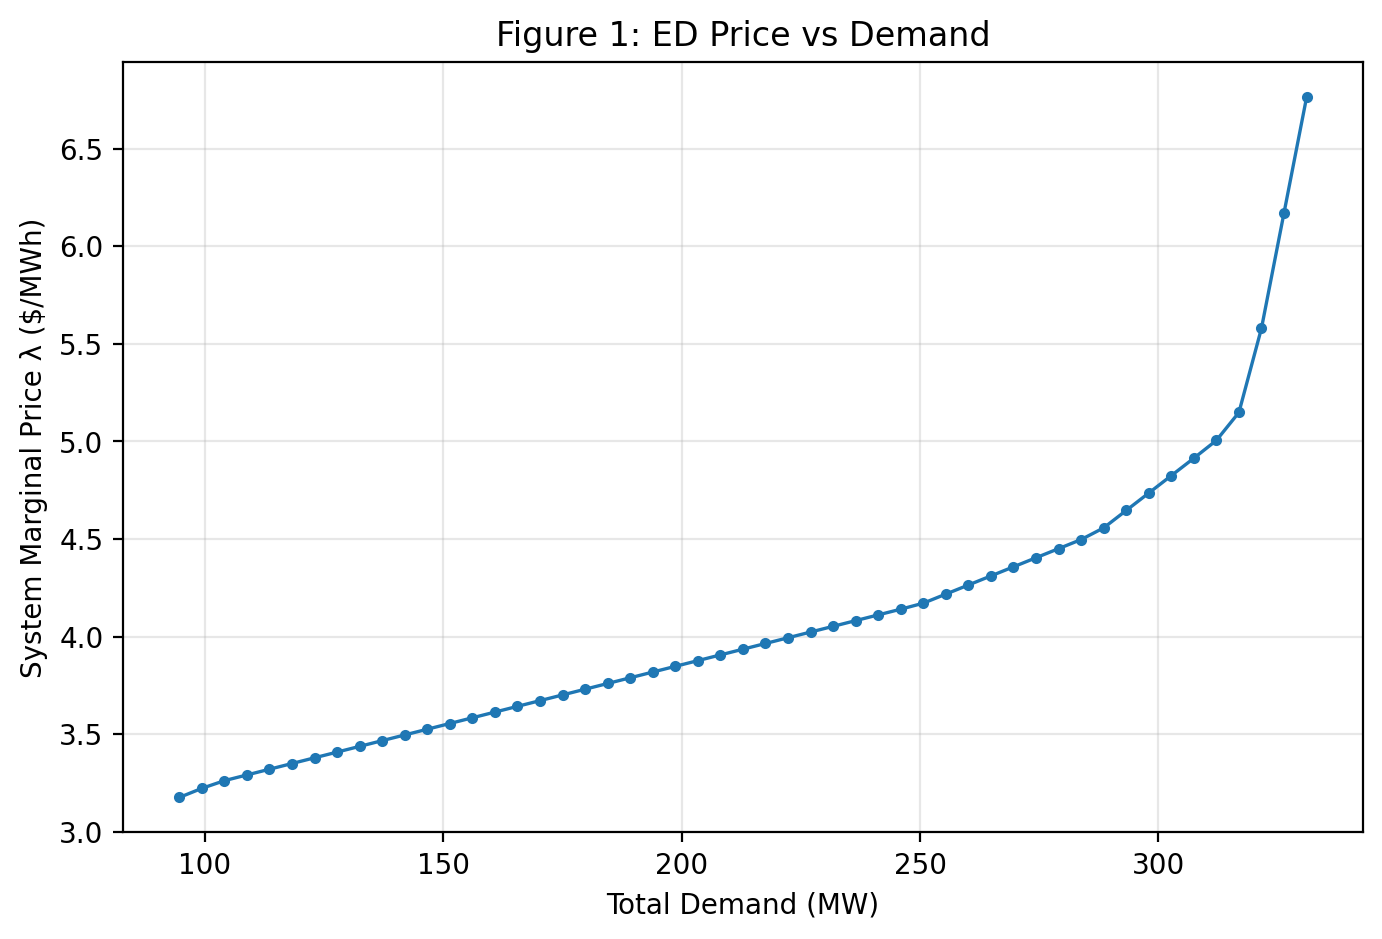
\includegraphics[width=0.85\textwidth]{fig1_price_vs_demand.png}
\caption{Economic Dispatch marginal price $\lambda$ vs.\ total demand, with generator limit transitions highlighted.}
\label{fig:price_demand}
\end{figure}

The marginal price curve exhibits distinct slope discontinuities (kinks) at specific demand thresholds where individual generators reach their maximum output capacity $P_{\max}$ and are clamped:
\begin{itemize}
    \item At $D = 260.15\text{ MW}$, Generator 4 reaches its upper limit $P_{\max, 4} = 55.0\text{ MW}$.
    \item At $D = 288.53\text{ MW}$, Generator 5 reaches $P_{\max, 5} = 30.0\text{ MW}$.
    \item At $D = 302.72\text{ MW}$, Generator 2 reaches $P_{\max, 2} = 80.0\text{ MW}$.
    \item At $D = 321.64\text{ MW}$, Generators 1 and 6 hit their respective bounds ($P_{\max, 1} = 80.0\text{ MW}$ and $P_{\max, 6} = 40.0\text{ MW}$).
    \item Generator 3 never reaches its capacity limit ($P_{\max, 3} = 50.0\text{ MW}$) within this demand range.
\end{itemize}
Whenever a generator reaches $P_{\max}$, it can no longer provide incremental energy. The system-wide incremental cost slope $\left(\sum_{i \notin \mathcal{A}} \frac{1}{2c_i}\right)^{-1}$ increases stepwise, steepening the price trajectory while preserving continuity in $\lambda$.

\subsection{Congestion Sweep and Locational Price Divergence}

Figure~\ref{fig:cost_spread} plots total operating cost and LMP spread as the line-rating scale factor is decreased from $1.000$ to $0.700$ in steps of $0.005$. Figure~\ref{fig:lmp_bus} shows the corresponding spatial distribution of LMPs across all 30 buses at selected ratings.

\begin{figure}[htbp]
\centering
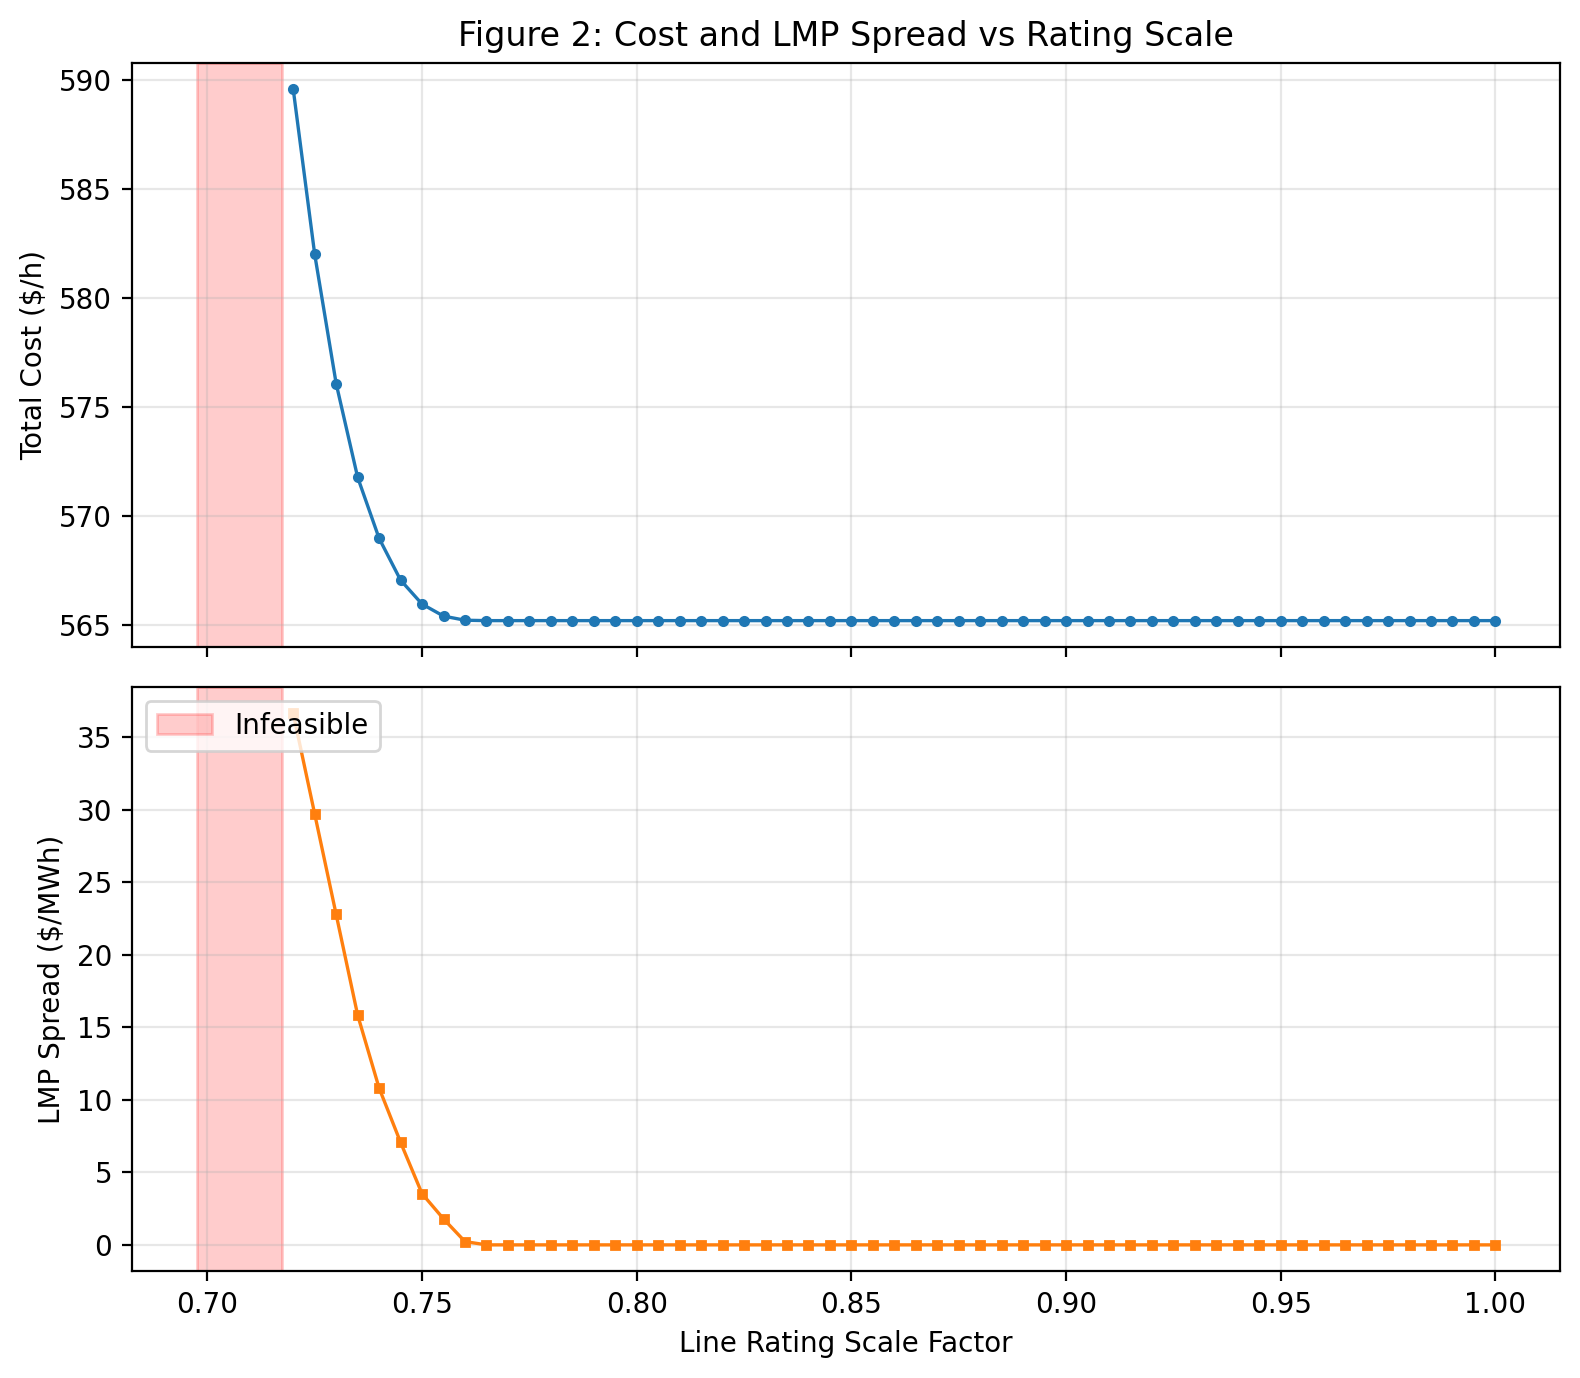
\includegraphics[width=0.85\textwidth]{fig2_cost_spread_vs_rating.png}
\caption{Total system operating cost and LMP spread vs.\ line rating scale factor.}
\label{fig:cost_spread}
\end{figure}

For ratings down to $0.765\times$, the network is completely uncongested; no line flows reach their limits, operating cost remains at $\$565.21\text{/h}$, and LMPs are uniform across all 30 buses ($\lambda = 3.7892\text{ \$/MWh}$). At rating scale $0.760$, line 6--8 becomes the first binding transmission constraint. To prevent line overload, the solver redispatches generation, causing system cost to rise to $\$565.22\text{/h}$ and LMPs to separate ($3.7885$ to $3.8117\text{ \$/MWh}$).

At rating scale $0.750$, two transmission lines bind simultaneously (branches 6--8 and 25--27). System cost increases to $\$565.97\text{/h}$, and the LMP spread widens from $3.6524$ to $7.1828\text{ \$/MWh}$. At rating scale $0.720$, four lines become constrained (branches 6--8, 15--23, 21--22, and 25--27), forcing extensive out-of-merit generation that elevates operating cost to $\$589.58\text{/h}$ and produces an extreme price spread of $3.0185$ to $39.6548\text{ \$/MWh}$.

\begin{figure}[htbp]
\centering
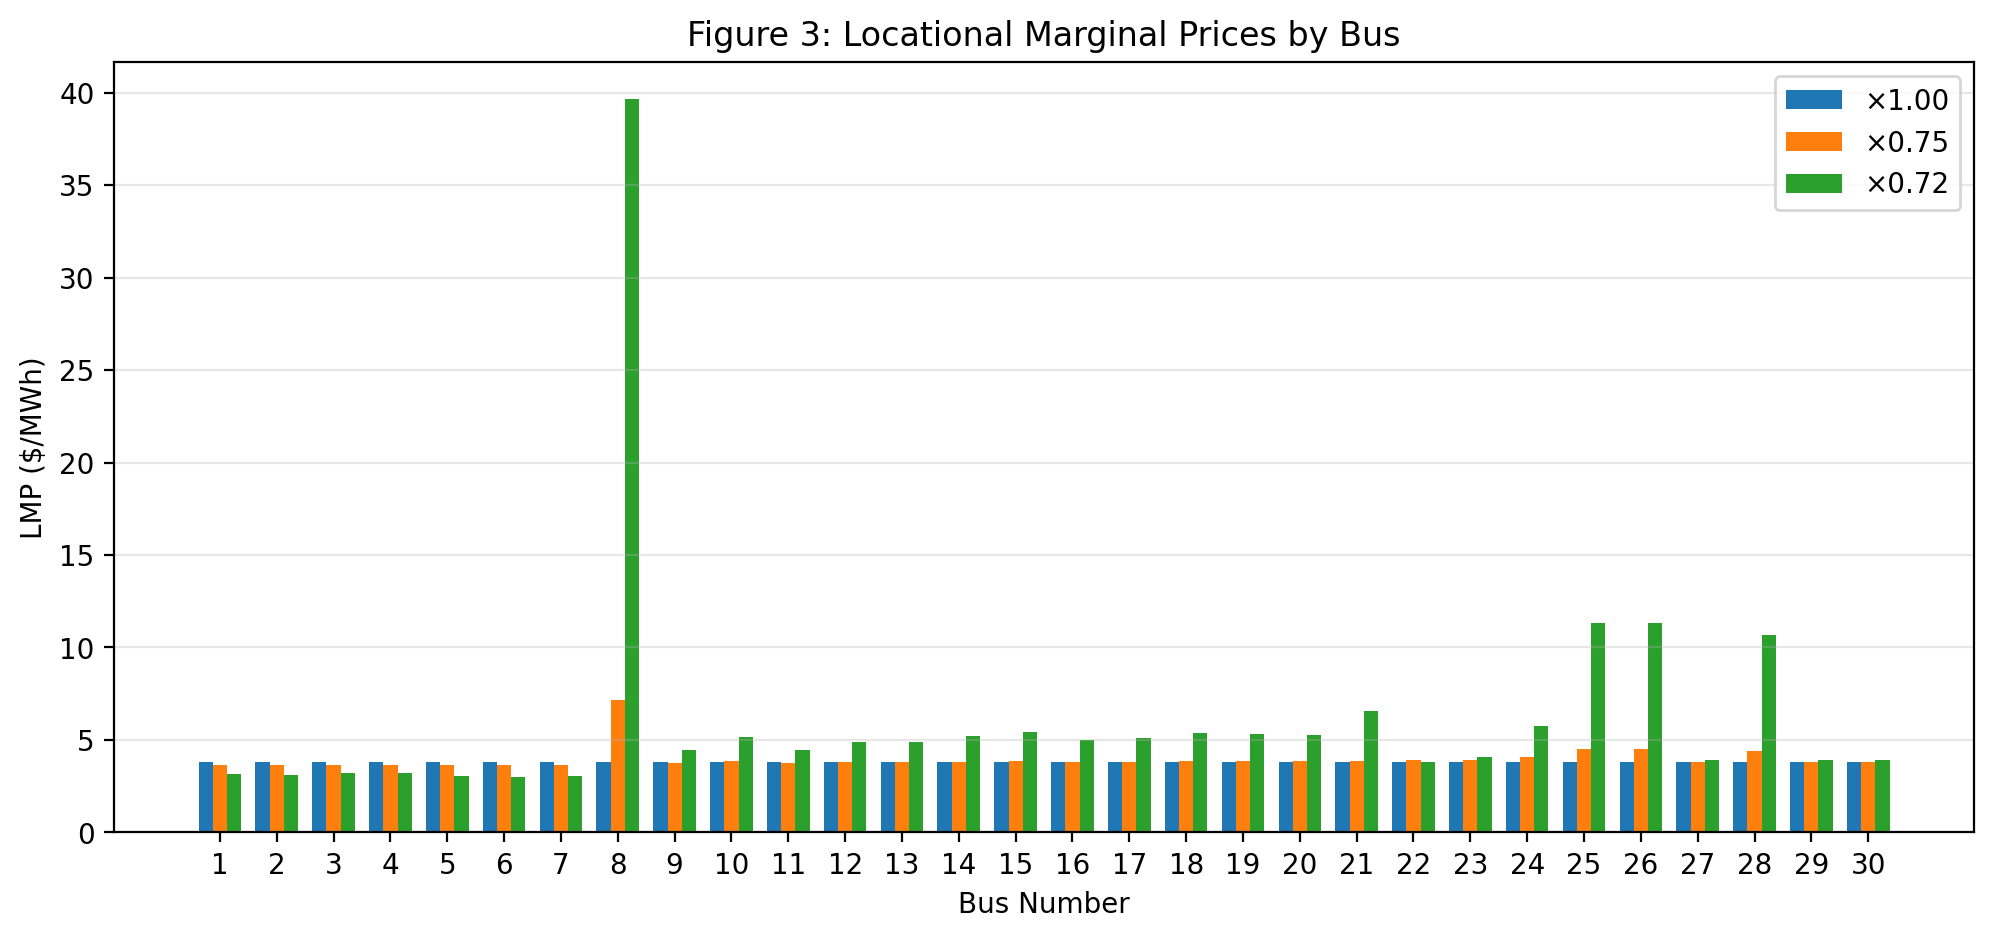
\includegraphics[width=0.95\textwidth]{fig3_lmp_per_bus.png}
\caption{Locational Marginal Prices by bus for rating scale factors 1.00, 0.75, and 0.72.}
\label{fig:lmp_bus}
\end{figure}

Bisection of the feasibility boundary demonstrates that the system becomes strictly infeasible below a line rating scale factor of $0.7167$. Below this threshold, transmission bottle-necks make it physically impossible to satisfy nodal power balances and generator capacity constraints simultaneously.

\subsection{Active-Set Convergence}

Figure~\ref{fig:convergence} displays the objective function values across iterations of the primal active-set solver when starting from non-optimal feasible initial points.

\begin{figure}[htbp]
\centering
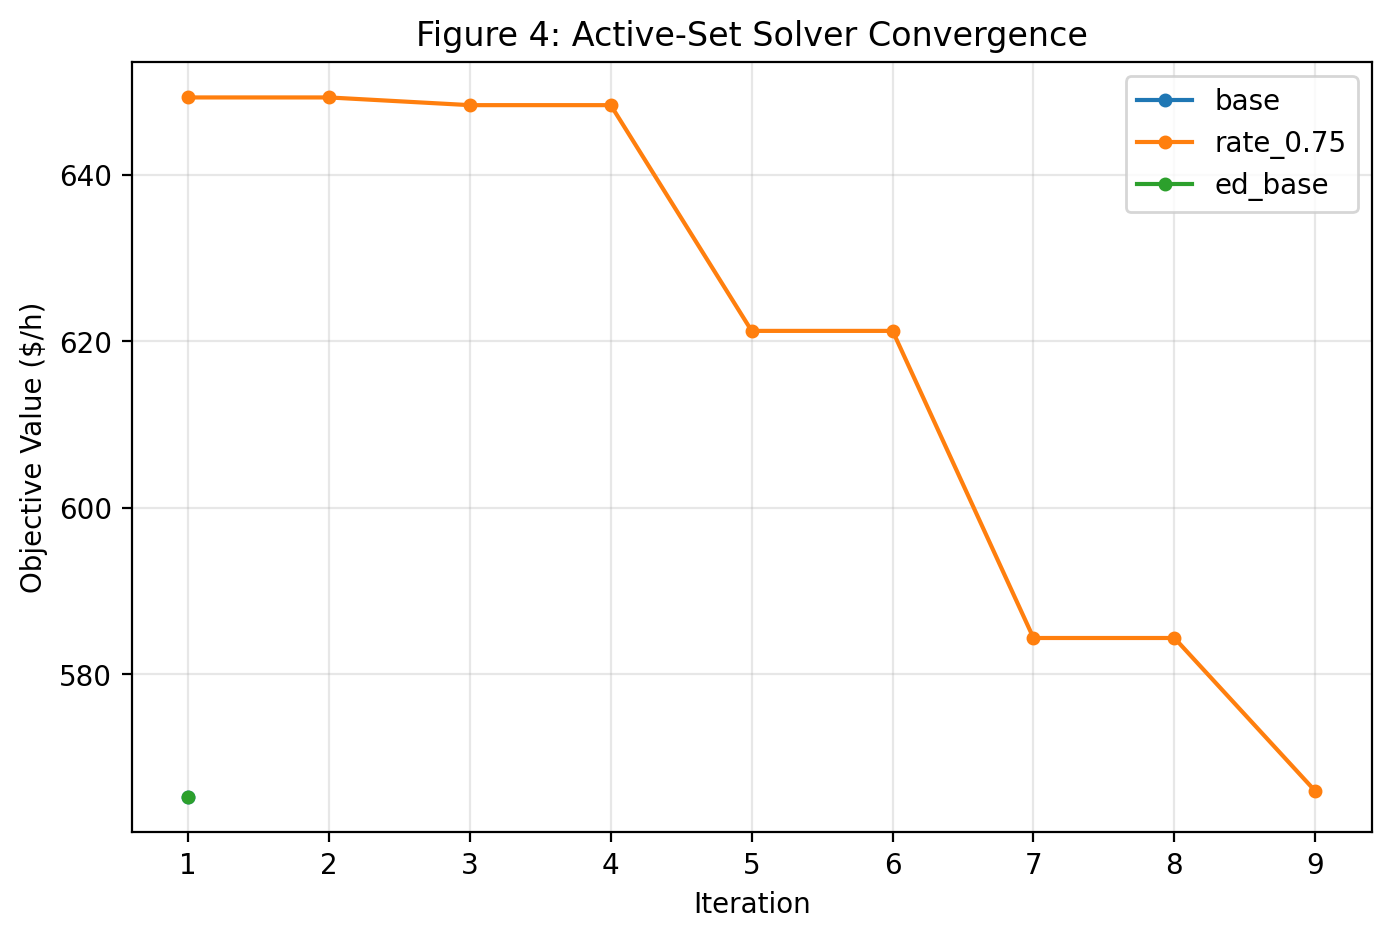
\includegraphics[width=0.85\textwidth]{fig4_active_set_history.png}
\caption{Primal active-set solver objective value per iteration from high-cost feasible initial points.}
\label{fig:convergence}
\end{figure}

In accordance with theoretical guarantees for Algorithm~16.3 \cite{nocedal2006}, the objective value decreases strictly monotonically at every iteration across all test scenarios. The uncongested base case converges in 13 iterations, the congested case ($0.75\times$) converges in 14 iterations after incorporating binding transmission constraints into the active set, and the ED case converges in 11 iterations. In each case, once the optimal active constraint manifold is identified, the subproblem step $p_k$ drops to zero, and dual multiplier non-negativity certifies optimality.


\end{document}
